\documentclass[12pt]{article}
\usepackage{amsmath,amssymb,amsthm}
\usepackage{tikz}
\usepackage{float}

\title{Othello Board Analogy for Collatz-Type Cycles}
\author{Jon Seymour}
\date{}

\begin{document}
\maketitle

\section{Introduction}

We study the realization of cycles in two-parameter Collatz-type maps using an Othello board analogy. Let
\[
T(x) =
\begin{cases}
g x + q, & x \text{ odd},\\
\dfrac{x}{h}, & x \equiv 0 \pmod h,
\end{cases}
\]
where \(g\) is odd, \(h \ge 2\), and \(q \in \mathbb{Z}\). For a cycle with \(o\) odd steps and \(e\) even steps, define
\[
d(g,h) = h^e - g^o
\]
and let \(k(g,h)\) encode the full parity structure of the cycle.

The fundamental \emph{cycle-element identity} is
\[
q\,k(g,h) - x_0 \, d(g,h) = 0.
\]

\subsection*{The polynomial \(p(g,h)\)}

Define
\[
p(g,h) = q\,k(g,h) - x_0 \, d(g,h),
\]
regarded as a bivariate polynomial in \(g\) and \(h\) with integer coefficients determined by \(q\), \(x_0\), and the cycle exponents \(o,e\). Then
\[
p(g,h) = 0 \quad \Longleftrightarrow \quad (g,h,q) \text{ admit a cycle with structure } k(g,h).
\]

\section{Othello Board Representation}

\subsection{Active Region}

The \emph{active region} of the board spans \(o+1\) columns and \(e+1\) rows. The horizontal coordinate \(j\) runs from the starting column \(-1\) to \(o-1\), and the vertical coordinate \(i\) runs from \(0\) to \(e\). This ensures the entire set of monomials in \(p(g,h)\) is represented, including the starting state at \(j=-1\).

\subsection{Pebble Placement}

For each monomial \(c_{j,i} g^{o-1-j} h^i\) in \(p(g,h)\):
\begin{itemize}
    \item Place a stack of \(c_{j,i}\) white pebbles if the coefficient is positive, black pebbles if negative.
    \item Each pebble sits in grid square \((j,i)\).  
\end{itemize}

\section{Conservation Laws}

\begin{enumerate}
    \item \textbf{Cancellation:} A black and white pebble on the same square may be removed simultaneously.
    \item \textbf{Column multiplication by \(g\):} A pebble may be exchanged for \(g\) pebbles of the same color on the right, or vice versa.
    \item \textbf{Row multiplication by \(h\):} A pebble may be exchanged for \(h\) pebbles of the same color below, or vice versa.
    \item \textbf{Special Collatz relations:}
    \begin{itemize}
        \item For 3x+1 systems (\(g = h^2-1\)), a white(/black) pebble at \((j,i)\) may be replaced by a white(/black) pebble at \((j+1,i+2)\) and a black(/white) pebble at \((j+1,i)\).
        \item For 5x+1 systems (\(g = h^2 + h -1\)), a white(/black) pebble at \((j,i)\) may be replaced by two white(/black) pebbles and one black(/white) pebble according to the three monomials in the identity.
    \end{itemize}
\end{enumerate}

\section{Worked Example: \(x = 17, g = 5, h = 2, q = 1\)}

\subsection{Polynomial}

The exact polynomial is
\[
p_{1093}(g,h) = 17 g^3 + g^2 q + g h q - 17 h^7 + h^4 q.
\]

\subsection{Othello Board Diagram}

\begin{figure}[H]
\centering
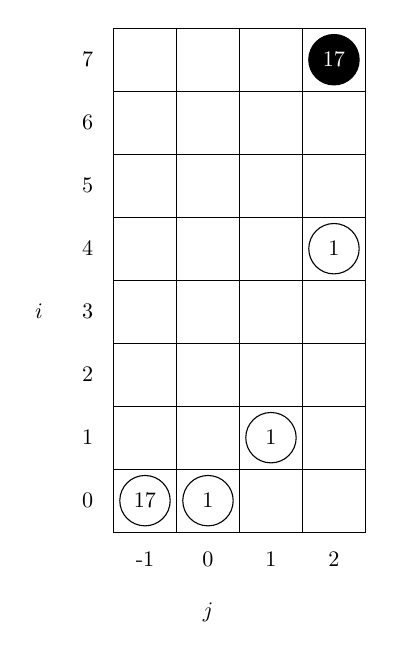
\begin{tikzpicture}[scale=0.8, every node/.style={scale=0.8}]
% Draw the grid: j=-1..2 (4 columns), i=0..7
\foreach \j in {-1,0,1,2} {
    \foreach \i in {0,1,2,3,4,5,6,7} {
        \draw (\j,\i) rectangle ++(1,1);
    }
}

% Label columns (x-axis) at bottom
\node[below] at (0.5,-1) {$j$};
\foreach \j in {-1,0,1,2} {
    \node[below] at (\j+0.5,-0.2) {\j};
}

% Label rows (y-axis) on left
\node[left] at (-2,3.5) {$i$};
\foreach \i in {0,1,2,3,4,5,6,7} {
    \node[left] at (-1.2,\i+0.5) {\i};
}

% Pebble drawing function
\newcommand{\pebble}[5]{ 
    \filldraw[fill=#3, draw=black] (#1+0.5,#2+0.5) circle (0.4);
    \node[text=#4] at (#1+0.5,#2+0.5) {#5};
}

% Place pebbles according to polynomial coordinates
\pebble{-1}{0}{white}{black}{17}  % 17 g^3
\pebble{0}{0}{white}{black}{1}    % g^2 q
\pebble{1}{1}{white}{black}{1}    % g h q
\pebble{2}{4}{white}{black}{1}    % h^4 q
\pebble{2}{7}{black}{white}{17}   % -17 h^7
\end{tikzpicture}
\caption{Othello board representation of $p_{1093}(g,h)$. Horizontal axis indexed by $j$, vertical axis by $i$. White pebbles with black numerals correspond to positive coefficients; black pebbles with white numerals correspond to negative coefficients.}
\label{fig:pebble-board}
\end{figure}

\subsection{Gameplay}

Gameplay proceeds by applying the conservation laws until:
\begin{itemize}
    \item All pebbles disappear (zero pebble state), corresponding to a cycle of the related Collatz system, or
    \item All remaining pebbles are of the same color (no further cancellation possible).
\end{itemize}

\section{Constraints on Initial State}

\begin{itemize}
    \item For all $j \in [0,o-1]$, $i \in [0,-1]$, any non-zero $c_{j,i}$ cannot "see" any other pebbles in its lower-right quadrant (including its own column and row).
    \item Inside this region, all stacks are of identical height and color.
    \item Every column in $[0,o-1]$ has the same non-zero number of pebbles.
\end{itemize}

\section{Conclusion}

The Othello board analogy provides a concrete visualization of the polynomial \(p(g,h)\) associated with Collatz-type cycles. Pebbles correspond to monomials, and conservation laws encode allowed transformations. The zeroing game then directly mirrors cycle realization in the underlying map.

\end{document}
